% Copyright 2004 by Till Tantau <tantau@users.sourceforge.net>.
%
% In principle, this file can be redistributed and/or modified under
% the terms of the GNU Public License, version 2.
%
% However, this file is supposed to be a template to be modified
% for your own needs. For this reason, if you use this file as a
% template and not specifically distribute it as part of a another
% package/program, I grant the extra permission to freely copy and
% modify this file as you see fit and even to delete this copyright
% notice. 

\documentclass{beamer}

\usepackage{blindtext}
\usepackage{tcolorbox}
\usepackage{soul}

\usepackage{amsmath}
\usepackage{amssymb}
\usepackage{amsthm}
\usepackage{amsfonts}

\makeatletter
\newcommand\xleftrightarrow[2][]{%
  \ext@arrow 9999{\longleftrightarrowfill@}{#1}{#2}}
\newcommand\longleftrightarrowfill@{%
  \arrowfill@\leftarrow\relbar\rightarrow}
\makeatother

\usefonttheme{professionalfonts} % using non standard fonts for beamer
\usefonttheme{serif} % default family is serif
%\usepackage{fontspec}
%\setmainfont{Liberation Serif}

% There are many different themes available for Beamer. A comprehensive
% list with examples is given here:
% http://deic.uab.es/~iblanes/beamer_gallery/index_by_theme.html
% You can uncomment the themes below if you would like to use a different
% one:
%\usetheme{AnnArbor}
%\usetheme{Antibes}
%\usetheme{Bergen}
%\usetheme{Berkeley}
%\usetheme{Berlin}
%\usetheme{Boadilla}
%\usetheme{boxes}
%\usetheme{CambridgeUS}
%\usetheme{Copenhagen}
%\usetheme{Darmstadt}
\usetheme{default}
%\usetheme{Frankfurt}
%\usetheme{Goettingen}
%\usetheme{Hannover}
%\usetheme{Ilmenau}
%\usetheme{JuanLesPins}
%\usetheme{Luebeck}
%\usetheme{Madrid}
%\usetheme{Malmoe}
%\usetheme{Marburg}
%\usetheme{Montpellier}
%\usetheme{PaloAlto}
%\usetheme{Pittsburgh}
%\usetheme{Rochester}
%\usetheme{Singapore}
%\usetheme{Szeged}
%\usetheme{Warsaw}



\title{Introduction to Signal Processing}

% A subtitle is optional and this may be deleted
\subtitle{Lecture 8: \textbf{Design and implementation of analog filters}}

\author{Sivakumar Balasubramanian}
% - Give the names in the same order as the appear in the paper.
% - Use the \inst{?} command only if the authors have different
%   affiliation.

\institute[Christian Medical College] % (optional, but mostly needed)
{
  \inst{}%
  Department of Bioengineering\\
  Christian Medical College, Bagayam\\
  Vellore 632002
}
% - Use the \inst command only if there are several affiliations.
% - Keep it simple, no one is interested in your street address.

\date{}
% - Either use conference name or its abbreviation.
% - Not really informative to the audience, more for people (including
%   yourself) who are reading the slides online

\subject{Lecture notes on signal processing}
% This is only inserted into the PDF information catalog. Can be left
% out.

% If you have a file called "university-logo-filename.xxx", where xxx
% is a graphic format that can be processed by latex or pdflatex,
% resp., then you can add a logo as follows:

% \pgfdeclareimage[height=0.5cm]{university-logo}{university-logo-filename}
% \logo{\pgfuseimage{university-logo}}

% Delete this, if you do not want the table of contents to pop up at
% the beginning of each subsection:
\AtBeginSubsection[]
{
  \begin{frame}<beamer>{Outline}
    \tableofcontents[currentsection,currentsubsection]
  \end{frame}
}

% Let's get started
\begin{document}
\setbeamertemplate{caption}{\raggedright\insertcaption\par}

\begin{frame}
  \titlepage
\end{frame}

% READING MATERIAL
\begin{frame}{Reading material}

\begin{itemize}
\item Sections 8.1-8.7 from reference [2]
\end{itemize}

\end{frame}

% FILTERS
\begin{frame}{Filters}

\begin{itemize}
\item A \textit{filter} is any system that suppresses or removes undesired information from some desired information.
\item In signal processing, we are mostly interested in selecting information that is restricted to a particular frequency band. The filters used for his purpose are \textit{frequency selective filters}.
\item All LTI system act as some sort of frequency selective filter, and will thus introduce some sort of amplitude and phase distortion (wanted or unwanted) to the input signal.
\item The amount of distortion introduced is given by the frequency response of the LTI system.
\end{itemize}
\end{frame}

% IDEAL FILTERS
\begin{frame}{Ideal frequency selective filters}

\begin{itemize}
\item Most often information of interest (signal) is confined to a particular frequency band , and is corrupted with unwanted information (noise) which occupies another frequency band.
\begin{figure}
\centering
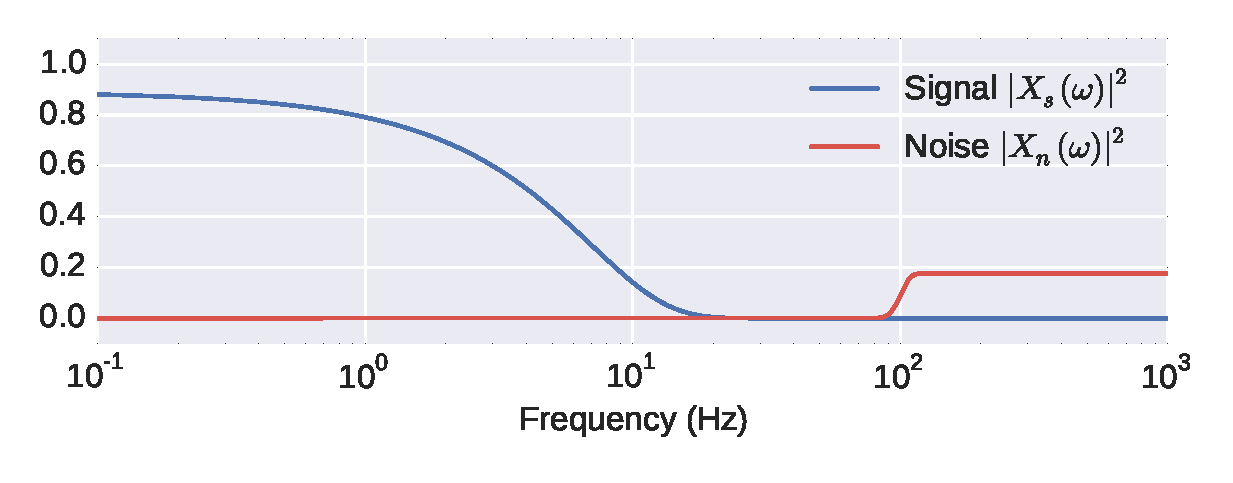
\includegraphics[width=0.8\textwidth]{img/sig_noise_sep.eps}
\end{figure}
\item One could separate the signal and the noise in this case by passing this signal through an LTI system that has non-zero magnitude response for the band of frequencies occupied by the signal, and zero magnitude response in the noise frequency band,

\end{itemize}
\end{frame}

% IDEAL FILTERS
\begin{frame}{Ideal frequency selective filters}
\begin{figure}
\centering
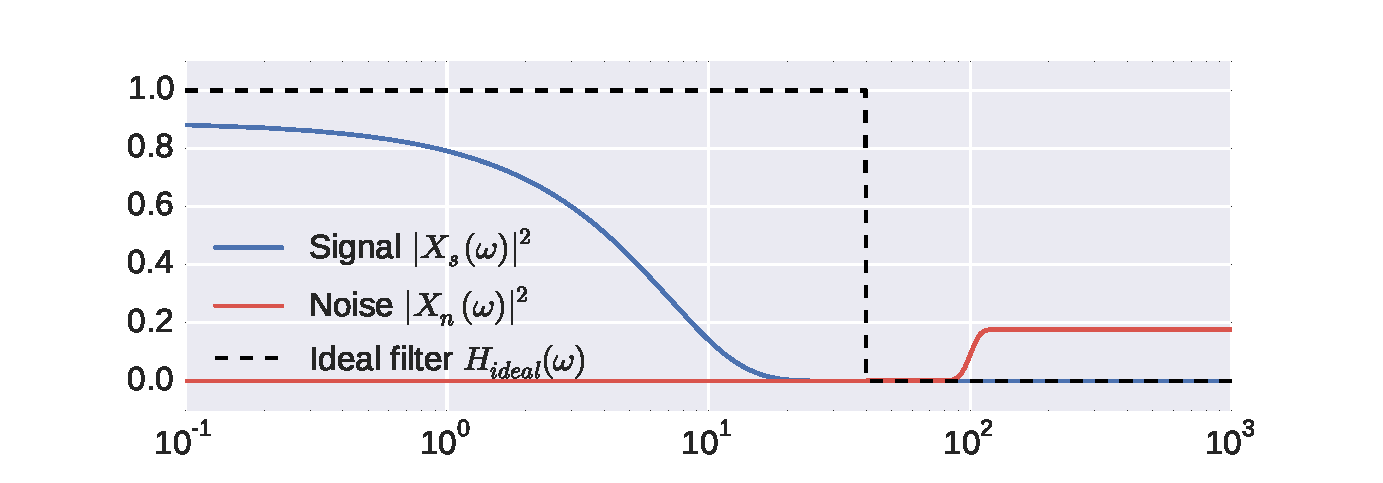
\includegraphics[width=0.8\textwidth]{img/sig_noise_ideal_filt.eps}
\end{figure}

\begin{small}
\begin{itemize}
\item Passing $X_s(j\omega) + X_n(j\omega)$ through $H_{ideal}\left(j\omega\right)$ will remove $X_n(j\omega)$ from the signal, and allow us to obtain $X_s(j\omega)$ undistorted.
\[ H_{ideal}(j\omega) = \begin{cases}
1 & |\omega| < \omega_c \\
0 & \text{Otherwise}
\end{cases} \implies h_{ideal}(t) =  \frac{\omega_c}{\pi}\frac{\sin \omega_c t}{\omega_c t}\]
\item $H_{ideal}(j\omega)$ is a non-causal system and thus cannot be realized. This is true of any piecewise constant frequency response.
\item However, for practical purpose $H_{idea}(j\omega)$ can be approximated by allowing deviations from the ideal response, which can lead to some distortion of $X_s(j\omega)$.
\end{itemize}
\end{small}
\end{frame}

% REAL FREQUENCY SELECTIVE FILTERS
\begin{frame}{Real frequency selective filters}
\begin{itemize}
\item Ideal frequency responses can be approximated by allowing deviations from the piecewise constant response, as depicted below.
\begin{figure}
\centering
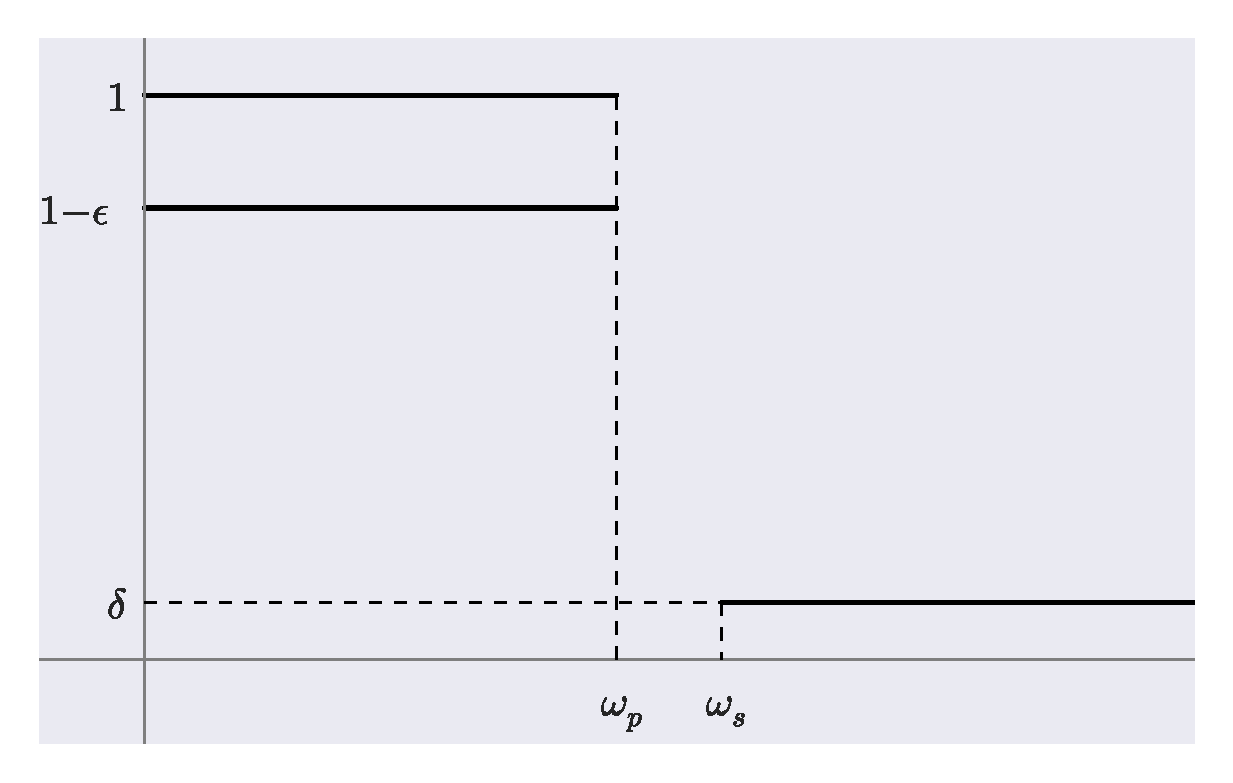
\includegraphics[width=0.6\textwidth]{img/real_filt.eps}
\end{figure}
\[\begin{cases}
1-\epsilon \leq |H(j\omega)| \leq 1, \,\,\, \forall |\omega| \leq \omega_p & \text{Passband} \\
|H(j\omega)| \leq \delta, \,\,\, \forall |\omega| \geq \omega_s & \text{Stopband} \\
\omega_p < |\omega| < \omega_p & \text{Transition band}
\end{cases} \]
\item $\omega_p$, $\omega_s$ are the \textit{passband and stopband cut-off frequencies}, and $\epsilon$ and $\delta$ are tolerance parameters. 
\end{itemize}
\end{frame}

% FOUR TYPES OF FREQUENCY SELECTIVE FILTERS
\begin{frame}{Four types of frequency selective filters}
\begin{figure}
\centering
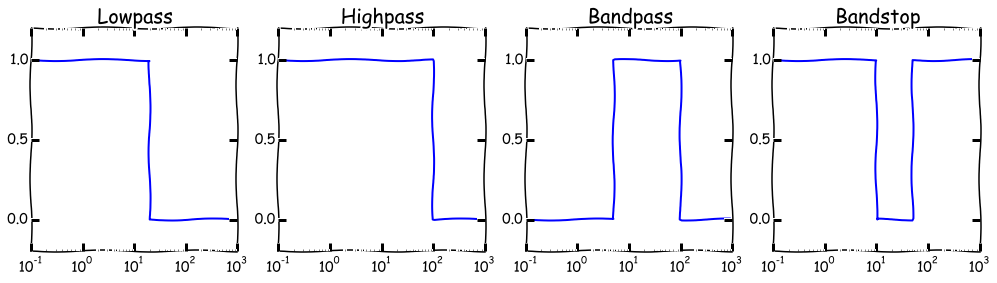
\includegraphics[width=\textwidth]{img/filters.png}
\end{figure}

Frequency selective filters can be broadly classified into four different types: \textit{lowpass}, \textit{highpass}, \textit{bandpass} and \textit{bandstop} filter.

The above figure shows the ideal responses of these four different filter types.

We will discuss in details the design of lowpass filters, which can be easily transformed into the other filter types.
\end{frame}

% REAL FREQUENCY SELECTIVE FILTERS
\begin{frame}{Real frequency selective filters}
\begin{itemize}
\item With these specifications the design of the filter is carried out in terms of the frequency response, rather than the impulse response.
\item The design of the filter then involves two steps:
\begin{itemize}
\item \textbf{Approximation}: involves coming with a rational transfer function whose frequency response satisfy the specifications. The rational transfer function must be both \textit{stable} and \textit{causal}.
\item \textbf{Realization}: involves the physical realisation of the rational transfer function with physical elements (resistors, inductors and capacitors for electrical systems, or springs, dampers and masses for mechanical systems).
\end{itemize}
\end{itemize}
\end{frame}

% APPROXIMATION
\begin{frame}{Approximation}
\begin{itemize}
\item The purpose of this step is to approximate the ideal frequency response using a rational transfer function $H(s)$, that is both stable and causal.
\[ H(s) = \frac{b_Ms^M + b_{M-1}s^{M-1} + \cdots + b_0}{a_Ns^N + a_{N-1}s^{N-1} + \cdots + a_0} \]
\item For $H(s)$ to be realizable:
\begin{itemize}
\item All the coefficients $\left\{a_i\right\}_{i=0}^N$ and $\left\{b_i\right\}_{i=0}^M$ must be real.
\item $a_i > 0, \,\,\, \forall i \in \left[0, 1, \ldots, N \right]$
\item $N \geq M$
\end{itemize}
\item The approximation step takes the filter specifications about a filter's magnitude response, and given use the coefficients $\left\{a_i\right\}_{i=0}^N$ and $\left\{b_i\right\}_{i=0}^M$, or the poles and zeros of the transfer function $H(s)$.
\end{itemize}
\end{frame}

% BILINEAR TRANSFER FUNCTION
\begin{frame}{Simple cases of $H(s)$: \textit{Bilinear} transfer function}
Consider a $H(s)$ of the following form,
\[ H(s) = \frac{b_1s + b_0}{a_1s + a_0} \]
This is called the \textit{bilinear} transfer function.\\
\vspace{2mm}

For any given transfer function, we can talk about transmission zeros, i.e. frequencies at which the $H(j\omega) = 0$. Transmission zeros are different from that of zeros, because a transfer function with no zeros can have transmission zeros at $\infty$.\\
\vspace{2mm}

Consider the following special case,
\[ H(s) = \frac{b_0}{a_1s + a_0} \]
$H(s)$ has a \textit{transmission} zero at $\infty$, as $\lim_{\omega \to \infty}H(j\omega) = 0$. 
\end{frame}

% BILINEAR TRANSFER FUNCTION
\begin{frame}{Simple cases of $H(s)$: \textit{Bilinear} transfer function}
Consider a $H(s)$ of the following form,
\[ H(s) = \frac{b_1s + b_0}{a_1s + a_0} \]

\textbf{Special cases}
\[\begin{cases}
\frac{b_0}{a_1s+a_0} & \,\,\,\text{Poles}: -\frac{a_0}{a_1};\,\,\,\text{Transmission Zeroes}: \infty \\
\frac{b_1s}{a_1s+a_0} & \,\,\,\text{Poles}: -\frac{a_0}{a_1};\,\,\,\text{Transmission Zeroes}: 0 \\
\end{cases}
\]
Which of these behave likes a lowpass filter, and which one like a highpass filter?\\
\vspace{2mm}

How does $H(s) = \frac{b_1s + b_0}{a_1s + a_0}$ behave when $\frac{b_0}{a_0} > \frac{b_1}{a_1}$ and $\frac{b_0}{a_0} < \frac{b_1}{a_1}$?
\end{frame}

% BIQUADRATIC TRANSFER FUNCTION
\begin{frame}{Simple cases of $H(s)$: \textit{Biquaratic} transfer function}
Consider a $H(s)$ of the following form,
\[ H(s) = \frac{b_2s^2 + b_1s + b_0}{a_2s^2 + a_1s + a_0} \]
$H(s)$ has two poles (P) and two transmission zeros (TZ).
\vspace{2mm}

\textbf{Special cases}
\[\begin{cases}
\frac{b_0}{a_2s^2+a_1s+a_0} & \,\,\,\text{P}: \frac{-a1\pm \sqrt{a_1^2 - 4a_2a_0}}{2a_2};\,\,\,\text{TZ}: \text{2 at } \infty \\
\frac{b_2s^2}{a_2s^2+a_1s+a_0} & \,\,\,\text{P}: \frac{-a1\pm \sqrt{a_1^2 - 4a_2a_0}}{2a_2}; \,\,\,\text{TZ}: \text{2 at } 0 \\
\frac{b_1s}{a_2s^2+a_1s+a_0} & \,\,\,\text{P}: \frac{-a1\pm \sqrt{a_1^2 - 4a_2a_0}}{2a_2}; \,\,\,\text{TZ}: \text{1 at } 0, \text{1 at } \infty \\
\frac{b_2s^2+b_0}{a_2s^2+a_1s+a_0} & \,\,\,\text{P}: \frac{-a1\pm \sqrt{a_1^2 - 4a_2a_0}}{2a_2}; \,\,\,\text{TZ}: \pm \sqrt{\frac{b_0}{b_2}} \\
\end{cases}
\]

What type of filters do these three special cases correspond to?
\end{frame}

% APPROXIMATION
\begin{frame}{Approximation}

The purpose of the discussion on  bilinear and biquadratic transfer functions was to give you an idea about the nature of the numerator and denominator polynomials of the transfer function for the different filter types.\\
\vspace{2mm}

Hopefully now by looking at a transfer function (and through knowledge of its poles and transmission zeros) you would be able to roughly say the type of filter represented by the transfer function.\\
\vspace{2mm}

We will now look at two different approximation procedures that are used to obtain rational transfer functions for the given filter specification:
\begin{itemize}
\item \textbf{Maximally flat} magnitude response
\item \textbf{Equiripple} magnitude response
\end{itemize}
\end{frame}

% BUTTERWOTH FILTER
\begin{frame}{Butteworth filter}

The squared magnitude response of a $N^{th}$ order Butterworth filter is given by,
\[ \left|H(j\omega)\right|^2 = \frac{1}{1+\left(\frac{\omega}{\omega_0}\right)^{2N}}  \]

Has a maximally flat response, which formally means the following,
\[ \frac{\partial^k}{\partial\omega^k}\left|H(j\omega)\right|^2 = 0, \,\,\, \forall k \in \left\{1,2,3, \ldots, 2N-1 \right\}\]

\end{frame}

% BUTTERWOTH FILTER
\begin{frame}{Butteworth filter: Properties}
\[ \left|H(j\omega)\right|^2 = \frac{1}{1+\left(\frac{\omega}{\omega_0}\right)^{2N}}  \]

\begin{itemize}
\item It is an all pole filter. All of its transmission zeros are at infinity.
\item $\left|H(0)\right| = 1$ for any given order $N$.
\item $\left|H(\omega_0)\right| = \frac{1}{\sqrt{2}}$, which corresponds to the -3dB point.
\item Has a roll-off of $-20N$dB in the stopband.
\end{itemize}
\vspace{-2mm}

\begin{figure}
\centering
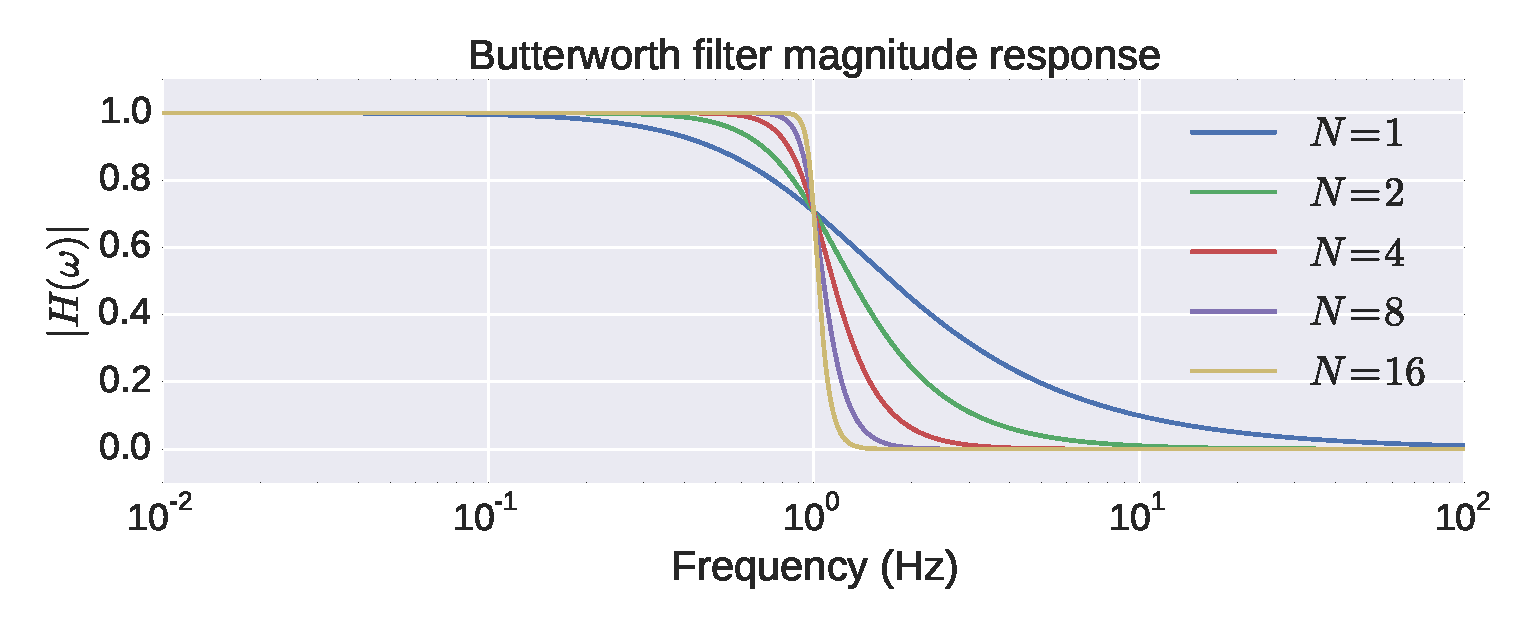
\includegraphics[width=\textwidth]{img/butter.eps}
\end{figure}
\end{frame}

% BUTTERWOTH FILTER
\begin{frame}{Butteworth filter: Properties}
\begin{small}
\[ \left|H(j\omega)\right|^2 = H(j\omega)H^*(j\omega) = H(j\omega)H(-j\omega) = H(s)H(-s)\bigg|_{s=j\omega} \]

\[\implies H(s)H(-s) = \frac{1}{1 + \left(\frac{s}{j\omega_0}\right)^{2N}} = \frac{1}{1 + \left(-1\right)^N\left(\frac{s}{\omega_0}\right)^{2N}} \]

\[ B_N(s)B_N(-s) = 1 + (-1)^N\left(\frac{s}{\omega_0}\right)^{2N} \]

$B_N(s)$ is the \textit{Butterworth polynomial}.

Let us consider the following cases to understand where the poles of $H(s)H(-s)$ are,
\[ N=1 \longrightarrow B_1(s)B_1(-s) = 1 - \left(\frac{s}{\omega_0}\right)^{2} = \left(1 - \frac{s}{\omega_0}\right)\left(1 + \frac{s}{\omega_0}\right) \]
The poles are at $\omega_0$ and $-\omega_0$.
\end{small}
\end{frame}

% BUTTERWOTH FILTER
\begin{frame}{Butteworth filter: Properties}
\begin{small}
\[ N=2 \longrightarrow B_2(s)B_2(-s) = 1 + \left(\frac{s}{\omega_0}\right)^{4} \,\,\,\, \text{Poles: } \omega_0e^{j(2k+1)\frac{\pi}{4}}, \,\,\, k = 0, 1, 2, 3 \]
\[ N=3 \longrightarrow B_3(s)B_3(-s) = 1 - \left(\frac{s}{\omega_0}\right)^{6} \,\,\,\, \text{Poles: } \omega_0e^{jk\frac{\pi}{3}}, \,\,\, k = 0, 1, \ldots 5 \]
In general, the poles of an $N^{th}$ order filter are located at,
\[ \begin{cases}
N \text{ is odd} & \longrightarrow \omega_0e^{jk\frac{\pi}{N}}, k = 0, 1, 2, \ldots 2N-1\\
N \text{ is even} & \longrightarrow \omega_0e^{j(2k+1)\frac{\pi}{2N}}, k = 0, 1, 2, \ldots 2N-1
\end{cases} \]

This means that the poles of $H(s)H(-s)$ are distributed on a circle of radius $\omega_0$.
\end{small}
\vspace{-5mm}

\begin{figure}
\centering
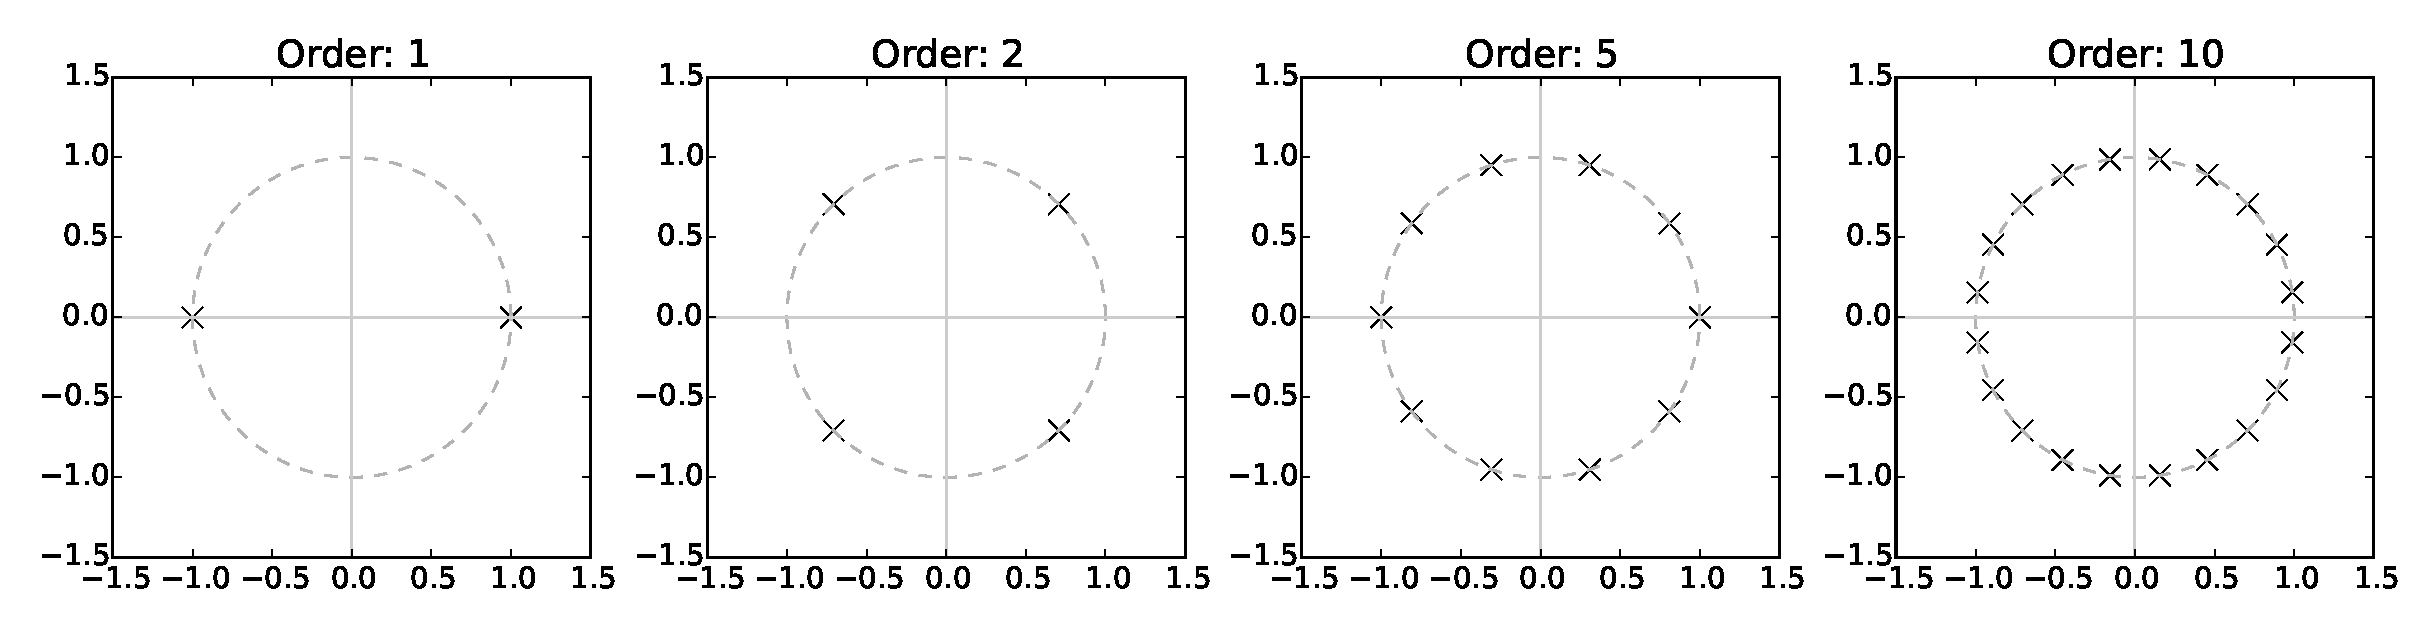
\includegraphics[width=1.1\textwidth]{img/butter_poles.eps}
\end{figure}
\end{frame}

% BUTTERWOTH FILTER
\begin{frame}{Butteworth filter: Properties}
Poles of $H(s)H(-s)$ are distributed on a circle of radius $\omega_0$.
\vspace{-5mm}
\begin{figure}
\centering
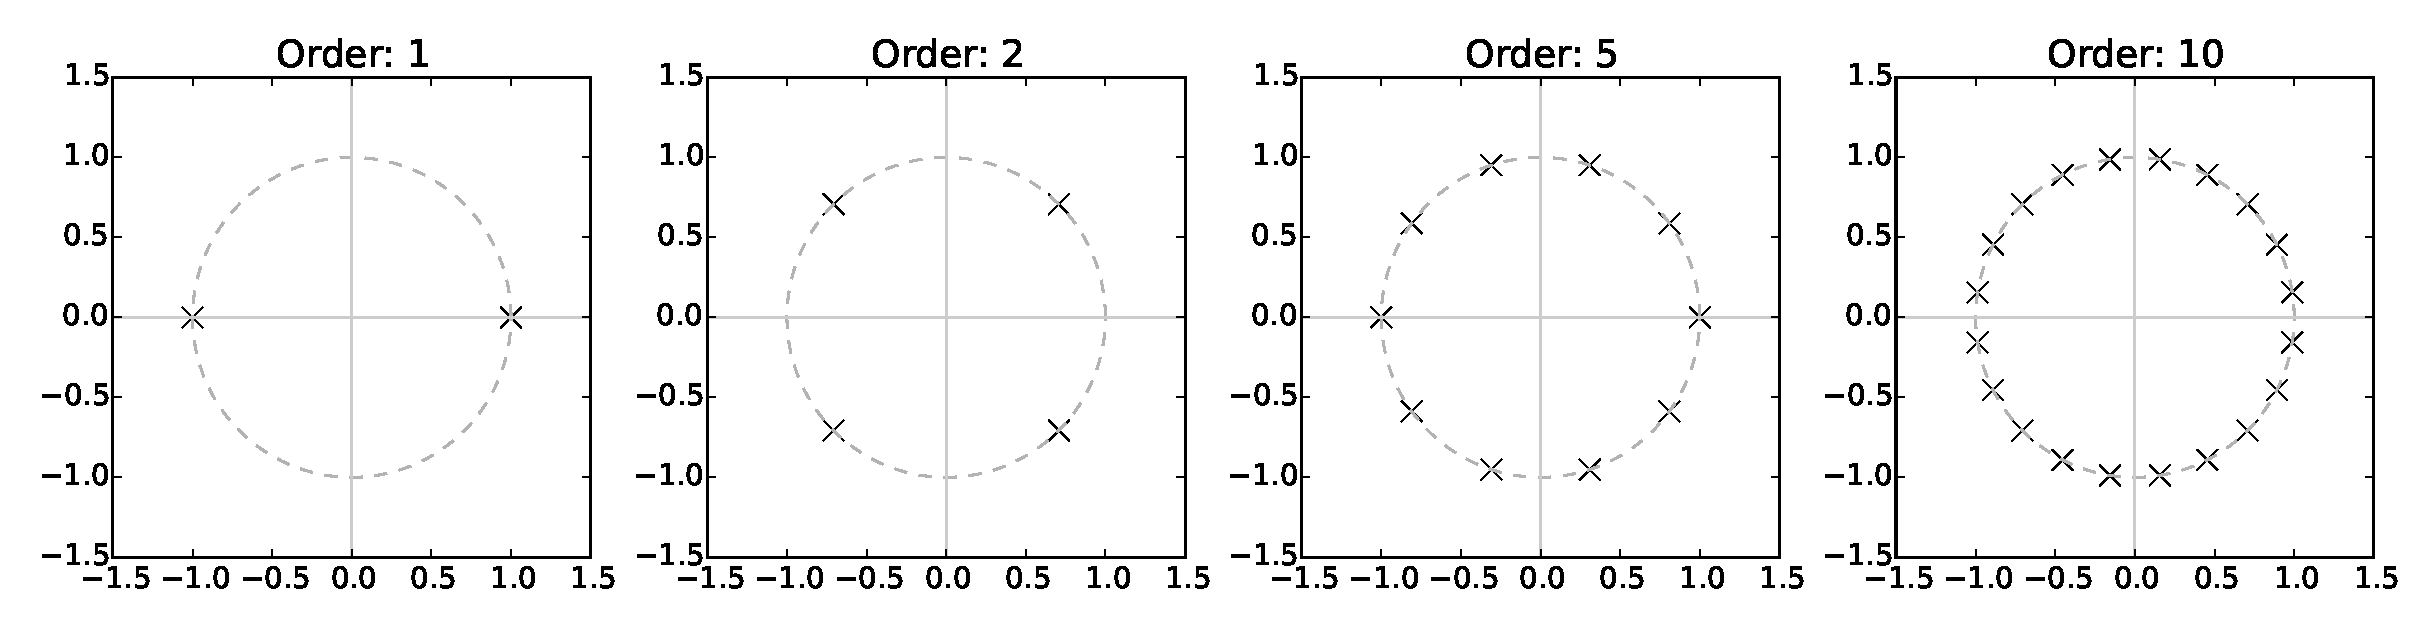
\includegraphics[width=1.\textwidth]{img/butter_poles.eps}
\end{figure}
\vspace{-5mm}
\begin{small}
A stable and causal filter can be implemented by choosing the poles on the left half of the $s$-plane, such that
\[ H(s) = \begin{cases}
N \text{ is even} & \longrightarrow \frac{1}{\Pi_{k}(s +2\omega_0\cos \phi_k s + \omega_0^2 p_i)} \\
N \text{ is odd} & \longrightarrow \frac{1}{\Pi_{k}(s+\omega_0)(s +2\omega_0\cos \phi_k s + \omega_0^2 p_i)} \\
\end{cases} \]

Where, $\phi_k$ is angle of the complex conjugate poles. $\phi_k$ can be found using the following simple rule.
\begin{enumerate}
\item $\phi_1 = \frac{N+1}{2N}\pi$
\item $\phi_k$ and $\phi_{k+1}$ are separated by $\frac{\pi}{N}$.
\end{enumerate}
\end{small}
\end{frame}

% DESIGN OF BUTTERWOTH FILTER
\begin{frame}{Design of Butteworth filter}
\begin{tiny}
\textbf{Filter design specifications:} $\epsilon=0.9, \delta = 0.1, \omega_p = 50\pi, \omega_s = 100\pi$. We need determine the values of Butterworth filter parameters $N$ and $\omega_0$ for the given specifications.
%\vspace{1mm}

The Butterworth magnitude response is given by, $\left|H(j\omega)\right|_{dB} = 20\log \left[1 + \left(\frac{\omega}{\omega_0}\right)^{2N}\right]^{-\frac{1}{2}} $
\vspace{-3mm}
\begin{equation}
\left|H(j\omega_p)\right|_{dB} = 20\log \epsilon = 20\log \left[1 + \left(\frac{\omega_p}{\omega_0}\right)^{2N}\right]^{-\frac{1}{2}} \implies \frac{1}{\epsilon^2} - 1 = \left(\frac{\omega_p}{\omega_0}\right)^{2N}
\label{eq:1}
\end{equation}
\vspace{-3mm}
\begin{equation}
\left|H(j\omega_s)\right|_{dB} = 20\log \delta = 20\log \left[1 + \left(\frac{\omega_s}{\omega_0}\right)^{2N}\right]^{-\frac{1}{2}} \implies \frac{1}{\delta^2} - 1 = \left(\frac{\omega_s}{\omega_0}\right)^{2N}
\label{eq:2}
\end{equation}
\vspace{-2mm}
\begin{equation}
\implies \frac{\left|H(j\omega_p)\right|_{dB}}{\left|H(j\omega_s)\right|_{dB}} = \frac{\frac{1}{\epsilon^2} - 1}{\frac{1}{\delta^2} - 1} = \left(\frac{\omega_p}{\omega_s}\right)^{2N} \implies N = \frac{1}{2}\frac{\log \left(\frac{\frac{1}{\epsilon^2} - 1}{\frac{1}{\delta^2} - 1}\right)}{\log \left(\frac{\omega_p}{\omega_s}\right)}
\label{eq:3}
\end{equation}
The order $N$ must be chosen as the lowest integer that is greater than the value obtained from Eq. \ref{eq:3}. Once the $N$ is determined, $\omega_0$ can be determined using Eq. \ref{eq:1} or Eq. \ref{eq:2}.
\[ \omega_0 = \frac{\omega_p}{\left(\frac{1}{\epsilon^2} - 1\right)^\frac{1}{2N}} \text{ or } \omega_0 = \frac{\omega_s}{\left(\frac{1}{\delta^2} - 1\right)^\frac{1}{2N}} \]

For the given specifications, 
\[ N = \frac{1}{2}\frac{\log \left(\frac{\frac{1}{0.9^2} - 1}{\frac{1}{0.1^2} - 1}\right)}{\log \left(\frac{10\pi}{15\pi}\right)} = 4.36 \implies N = 5\]
\[ \omega_0 = \frac{10\pi}{\left(\frac{1}{0.9^2}-1\right)^{\frac{1}{10}}} = 181.590 \]
\end{tiny}
\end{frame}

% DESIGN OF BUTTERWOTH FILTER
\begin{frame}{Design of Butteworth filter}
\begin{tiny}
\textbf{Filter design specifications:} $\epsilon=0.9, \delta = 0.1, \omega_p = 50\pi, \omega_s = 100\pi$.

Butterworth filter parameters: $N=5$, and $\omega_0=36.318$
\[ H(s) = \frac{1}{(s+181.59)\left(s^2+2(181.59)\cos \left(\frac{3\pi}{5}\right)+181.59^2\right)\left(s^2+2(181.59)\cos \left(\frac{4\pi}{5}\right)+181.59^2\right)} \]
\end{tiny}
%\vspace{-5m}

\begin{figure}
\centering
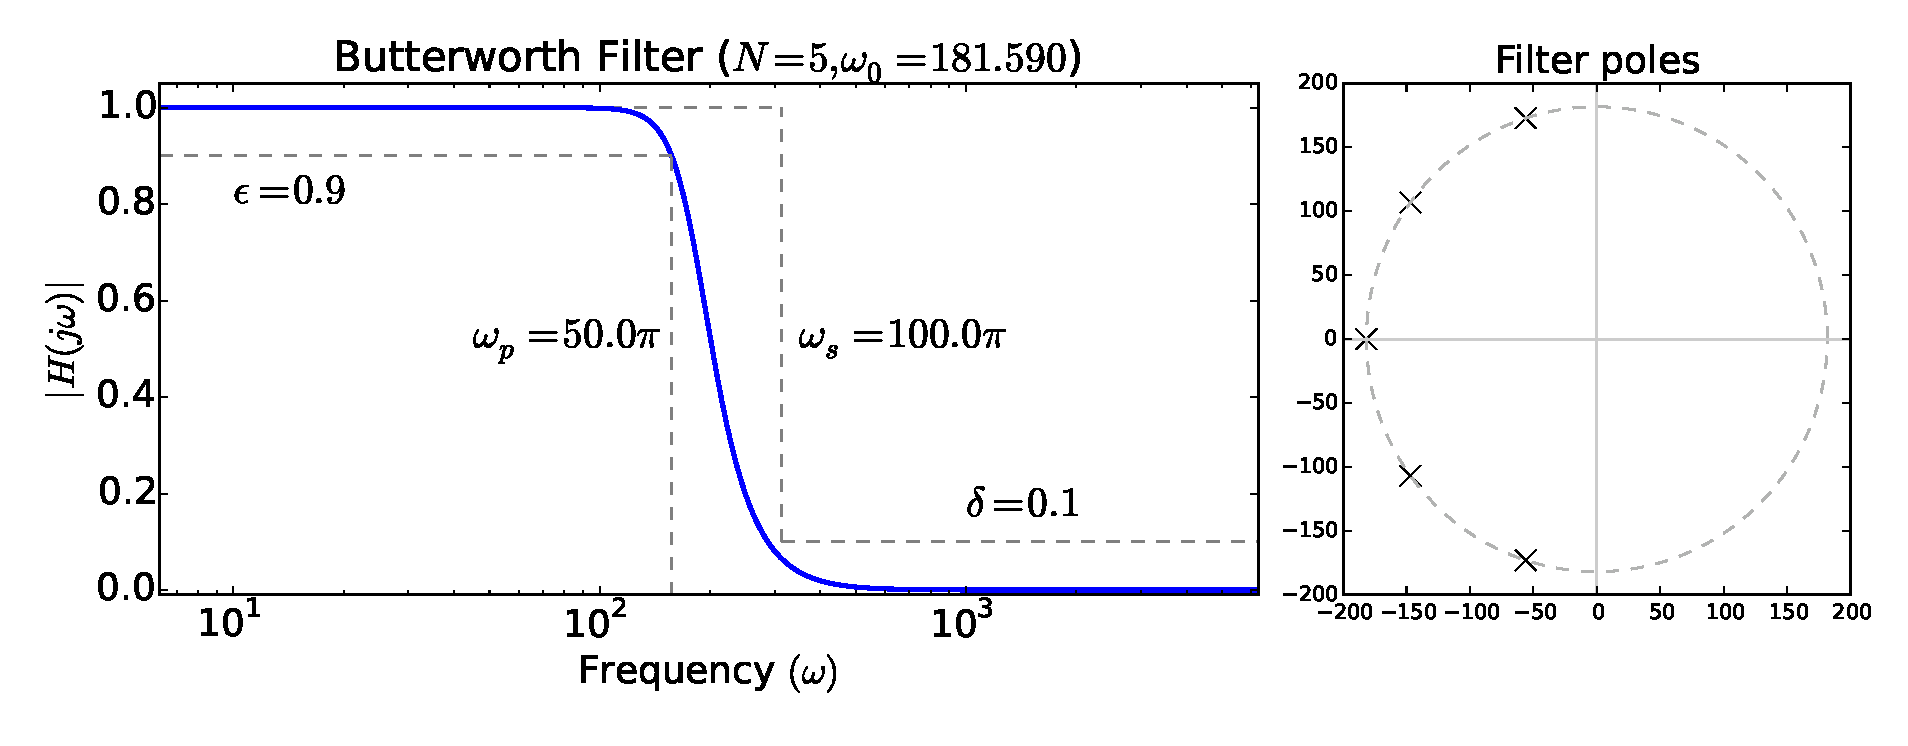
\includegraphics[width=\textwidth]{img/butter_filt_example.eps}
\end{figure}
\end{frame}

% CHEBYSHEV FILTER
\begin{frame}{Chebyshev filter}
\begin{small}
The Butterworth filter outperforms the filter specification in the passband, because of its monotonic response as a function of the frequency $\omega$.

The Chebyshev filter (an example of a equiripple filter) makes use of the specifications to give a filter with a lower order, by allowing the mangitude response to have ripples in the passband.

The squared magnitude response of a $N^{th}$ order Chebyshev filter is given by,
\[ \left|H(j\omega)\right|^2 = \frac{1}{1+\gamma^2C_N^2(\omega/\omega_0)} \]

where, $N$ is the order of the filter, $C_N(\bullet)$ is the \textit{Chebyshev polynomial}, and $1/\sqrt{1+\gamma^2}$ is the value of $|H(j\omega_0)|$.

\[ C_N\left(\omega\right) = \begin{cases}
\cos \left(N \cos^{-1} \omega\right) & \left|\omega\right| < 1 \\
\cosh \left(N \cosh^{-1} \omega\right) & \left|\omega\right| \geq 1 \\
\end{cases} \]
\end{small}
\end{frame}

% CHEBYSHEV FILTER
\begin{frame}{Chebyshev filter}
\[ \left|H(j\omega)\right|^2 = \frac{1}{1+\gamma^2C_N^2(\omega/\omega_0)} \]

\begin{figure}
\centering
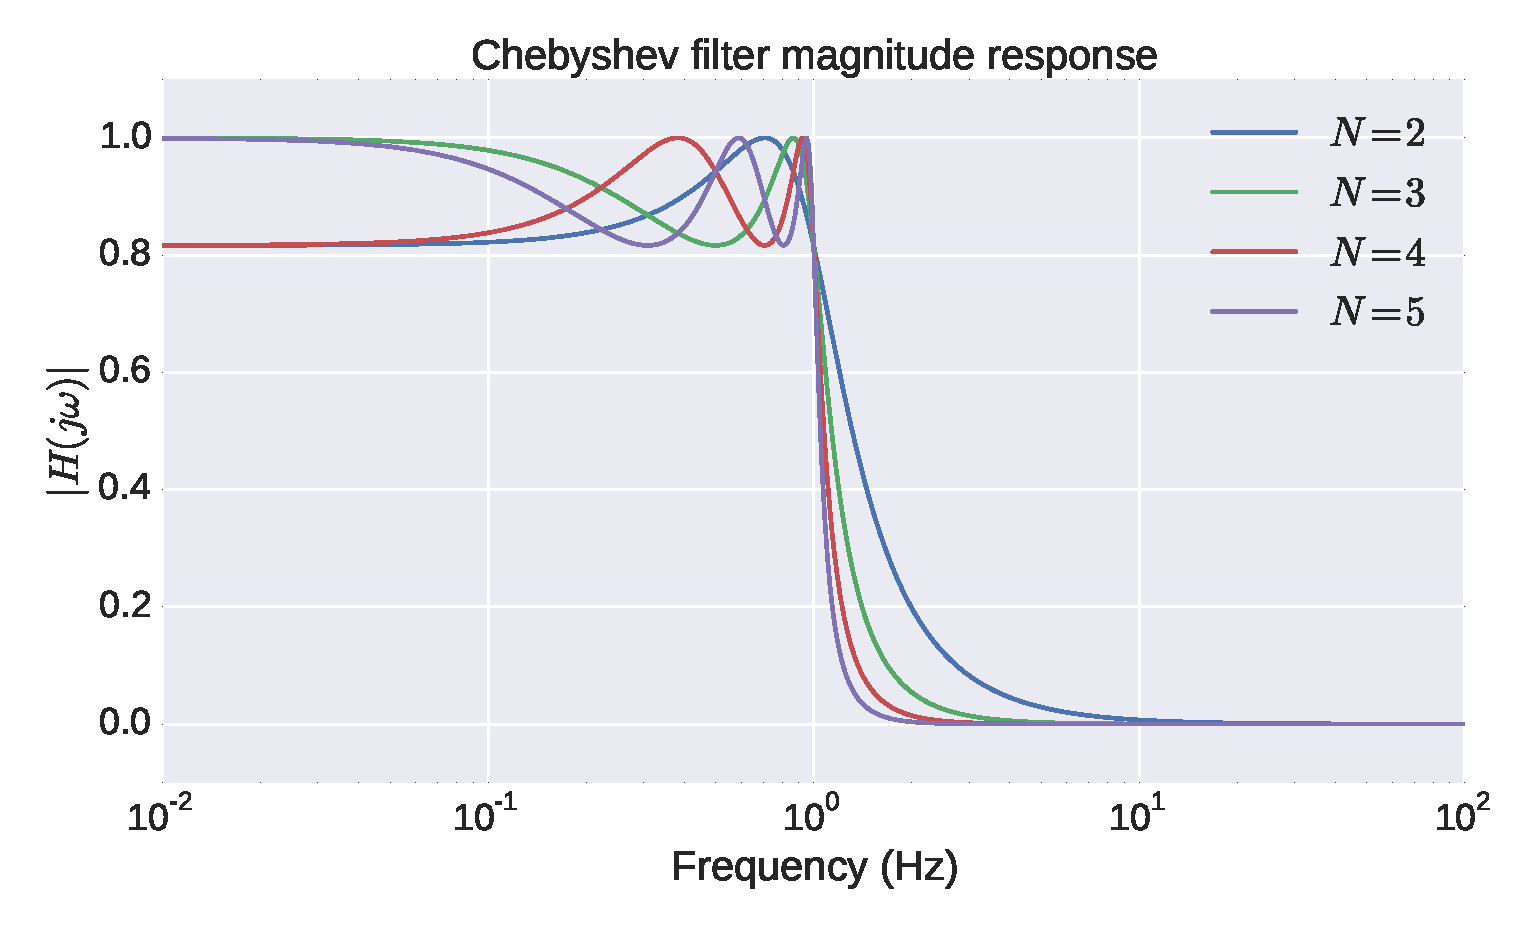
\includegraphics[width=\textwidth]{img/cheby.eps}
\end{figure}
\end{frame}

% DESIGN OF CHEBYSHEV FILTER
\begin{frame}{Design of Chebyshev filter: Properties}
\begin{tiny}
\textbf{Filter design specifications:} $\epsilon=0.9, \delta = 0.1, \omega_p = 50\pi, \omega_s = 100\pi$. 

We need determine the values of Chebyshev filter parameters $N$, $\gamma$ and $\omega_0$ for the given specifications.
%\vspace{1mm}

The Chebyshev magnitude response is given by, $H(j\omega) = \left[1 + \gamma^2C_N^2(\omega/\omega_0)\right]^{-\frac{1}{2}} $.

In the case of the Chebyshev filter, the value of $\omega_0$ is equal to $\omega_p$, which implies that,
\vspace{-1mm}
\begin{equation}
\epsilon^2 = \frac{1}{1 + \gamma^2} \implies \gamma = \sqrt{\frac{1}{\epsilon^2}-1}
\label{eq:4}
\end{equation}
\vspace{-2mm}
\begin{equation}
\left|H(j\omega_s)\right| = \delta = \left[1 + \gamma^2C_N^2(\omega_s/\omega_0)\right]^{-\frac{1}{2}} = \left[1 + \gamma^2\left(\cosh \left(N\cosh^{-1} (\omega_s/\omega_0)\right)\right)^2\right]^{-\frac{1}{2}}
\label{eq:5}
\end{equation}
\vspace{-2mm}
\begin{equation}
N = \frac{\cosh^{-1}\sqrt{\frac{\frac{1}{\delta^2} -1}{\gamma^2}}}{\cosh^{-1} (\omega_s/\omega_0)}
\label{eq:6}
\end{equation}

The order $N$ must be chosen as the lowest integer that is greater than the value obtained from Eq. \ref{eq:6}.

For the given specifications, 
\[ \gamma = \sqrt{\frac{1}{0.9^2} - 1} = 0.484 \,\,\, \text{ and } \,\,\, \omega_0 = \omega_p = 50\pi \]
\[ N = \frac{\cosh^{-1}\sqrt{\frac{\frac{1}{0.1^2} -1}{0.484^2}}}{\cosh^{-1} (100\pi/50\pi)} = 2.82 \implies N = 3 \]
\end{tiny}
\end{frame}

% DESIGN OF CHEBYSHEV FILTER
\begin{frame}{Design of Chebyshev filter}
\begin{tiny}
\textbf{Filter design specifications:} $\epsilon=0.9, \delta = 0.1, \omega_p = 50\pi, \omega_s = 100\pi$.

Chebyshev filter parameters: $N=3$, $\omega_0=157.080$ and $\gamma = 0.484$.
Note that the Chebyshev filter has resulted in a lower order than the corresponding Butterworth filter for the same specifications.
\end{tiny}
%\vspace{-5m}

\begin{figure}
\centering
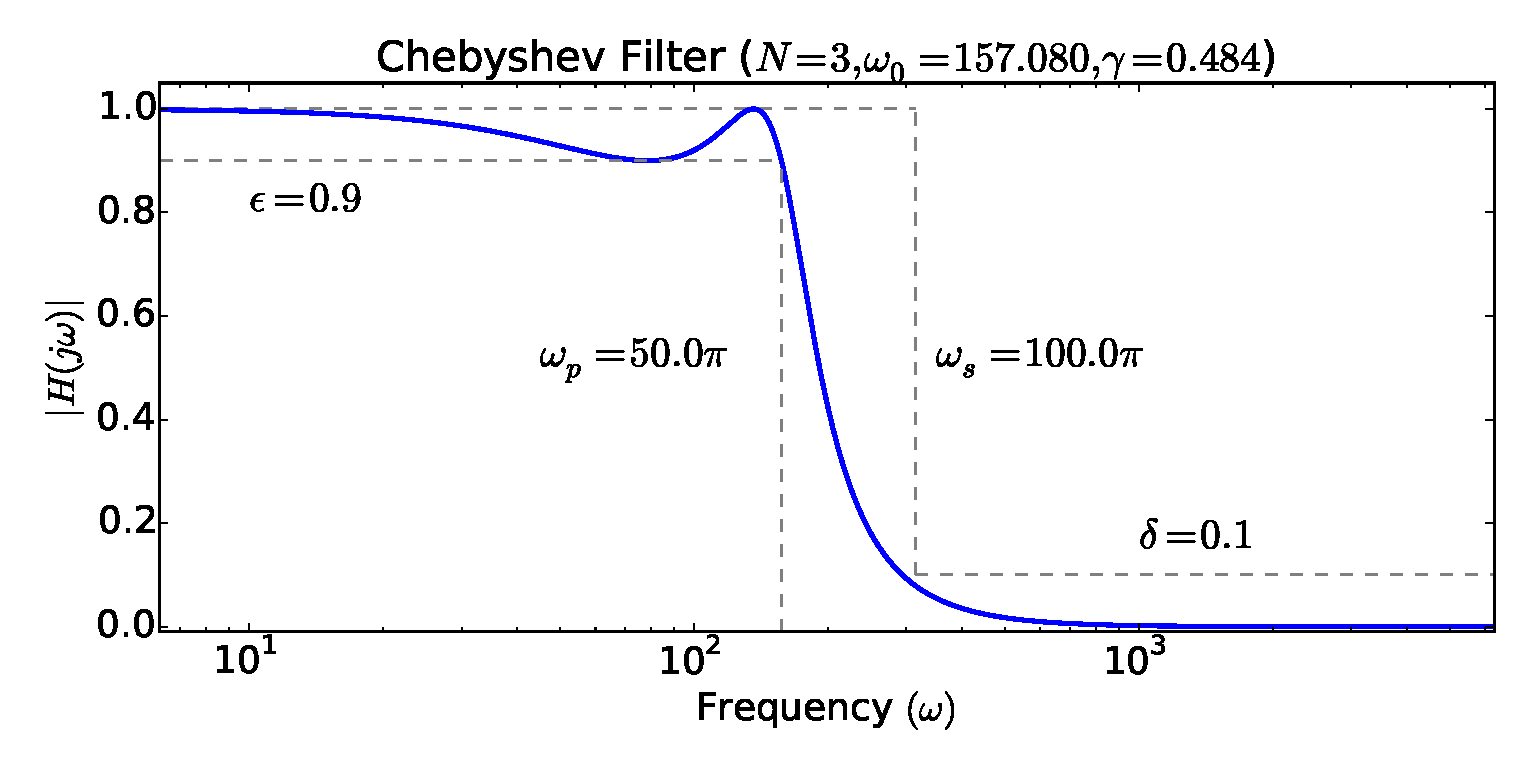
\includegraphics[width=\textwidth]{img/cheby_filt_example.eps}
\end{figure}
\end{frame}

% FREQUENCY TRANSFORMATIONS
\begin{frame}{Frequency transformations}
\begin{itemize}
\item We have so far only focused on the design of lowpass filter. This is because, a lowpass filter can be converted to another type (such a highpass, bandpass or bandstop) through an appropriate frequency transformation.
\item Given a lowpass transfer function $H_{0}(S)$, a frequency transformation procedure will replace the independent  In a frequency transformation, the independent variable $S$ is replaced by another variable $S=f(s)$, such that $H(s) = H_{0}(f(s))$ is the transformed filter (highpass, bandpass or bandstop) of interest.
\end{itemize}
\end{frame}

\end{document}